\documentclass[11pt]{article} % do not change this line
\input{BigDataStyle.txt}      % do not change this line
\usepackage{amsmath,amsfonts,amssymb,amsthm,latexsym,graphicx}
\usepackage{url}
\usepackage{multirow}

\emergencystretch=5mm
\tolerance=400
\allowdisplaybreaks[4]

\graphicspath{ {./images/} }

\theoremstyle{plain}
\newtheorem{theorem}{Theorem}[section]
\newtheorem{proposition}[theorem]{Proposition}
\newtheorem{corollary}[theorem]{Corollary}
\newtheorem{lemma}[theorem]{Lemma}
\newtheorem{problem}[theorem]{Problem}

\theoremstyle{definition}
\newtheorem*{remark}{Remark}

\title{Using Deep Learning for X-Ray Image Classification}
\author{Michael Harrison}

\newcommand{\Programme}{Machine Learning}
% Computational Finance students: uncomment the next line
%\twodepartmentstrue

\begin{document}
\maketitle

\declaration

\begin{acknowledgement}
I would like to thank...
\end{acknowledgement}

% NB: The abstract environment also inserts the Table of Contents
\begin{abstract}
ABSTRACT TBD
\end{abstract}


% BEGIN INTRODUCTION
\newpage
\setcounter{page}{1}
\pagenumbering{arabic}
\section{Introduction}
The aim of this project is to explore the use of Deep Learning in a practical situation. Deep Learning techniques have been used in a range of problems, such as image recognition [ref GoogleLeNet], natural language processing [ref Google Neural Machine Translation], playing games [ref AlphaGo] and self-driving cars [ref WayMo], among others. These techniques have often achieved cutting-edge performance on these tasks - for instance, surpassing human performance in the ImageNet task [ref ILSVRC], or beating the world champion Lee Sedol at the game Go [ref AlphaGo win]. As such, Deep Learning is an exciting branch of Machine Learning with the potential to make significant impacts in many areas of life. Indeed Deep Learning is one of (the?) largest areas of active research in Machine Learning at the time of writing [ref numbers of citations].
\\
\\
\noindent
This project focuses on image recognition, as this is one of the areas where Deep Learning has seen its biggest successes. In particular, we will be applying Deep Learning to the MURA (\textbf{mu}sculoskeletal \textbf{ra}diographs) dataset, published by the Machine Learning Group at Stanford University \cite{MURA2017}. This is a collection of 40,005 X-ray images of a part of the upper extremity - comprising the arm, shoulder, wrist, hand etc. Each image is from one of 14,656 studies of an individual patient, performed at a particular point in time on one of these parts of the upper extremity. Each study was labelled as normal or abnormal at the time of clinical interpretation by a radiologist from Stanford Hospital - and these labels have been published alongside the images themselves. Therefore the aim of this project is to use Deep Learning to perform binary image classification on this set of X-rays - classifying them as either normal or abnormal. This will be a supervised learning task, since we have clear labels for our data, and our aim is to predict them. 
\\
\\
\noindent
While any model developed as part of this project can only represent a toy solution to this problem, the principle of combining Deep Learning and medicine seems to be a good one. Inded this too is an area of active research, both within radiology [ref radiology], medical imaging [ref other DL/med image work] and medicine more widely [ref DL/med work]. The works cited of course represents only a small fraction of what is being done. Thinking optimistically, Deep Learning can help improve patient outcomes, produce results more quickly, alleviate pressure off medical pracitioners, reduce medical mistakes and improve medical decision-making. As such, this represents good motivation for me to dip my toe into this area as part of my project.

% END INTRODUCTION


% BEGIN BACKGROUND
\newpage
\section{Background}
This section describes the background of Deep Learning, and the methodology behind the techniques used in this project.

\subsection{Deep Learning}
The main idea behind Deep Learning is for a system to learn representations of the data given to it. While these representations can start out simple, they are organised into a hierarchical sequence of layers so that simpler representations from earlier layers can be composed and built up into higher-level, more complex representations. This is repeated over many layers so that the final representations have sufficient information and detail for the task at hand. This process of building up complex representations from simpler parts means that feature engineering - the choice of which aspects of the data to include in the model, how they should be transformed or combined etc - is performed automatically by the system, as part of training. This is one of the great strengths of Deep Learning since feature engineering as a manual process can be difficult and time-consuming, especially when the data is very high-dimensional (as with images).       

\subsection{Artificial Neural Networks}
\subsubsection{Basic Structure}
More specifically, these Deep Learning systems tend to be artificial neural networks (ANN's), of various forms depending on the nature of the task. A simple version of such a network \cite{wiki:simple_ann} is shown in \textbf{Figure \ref{fig:simple_ann}} below. These consist of a set of "neurons" (the circles in the image below) organised into layers, with each neuron from one layer connected to all neurons in the next layer. Each neuron has an associated activation, typically just a real number, which is derived from the activations of the neurons feeding into it from the previous layer. The input layer is a special case, where the neuron activations represent values from the item of data being fed into the network. For instance, for greyscale images, the input neurons correspond to each pixel in the given input image, and the input activations are simply each pixel's value. The activations of the final output layer may represent different things, depending on the task - for instance, the final learned representation of the data item when doing dimension reduction. Or, for classification, the probability distribution over the set of classes that captures the network's prediction of which class the given data item is in. 
\begin{figure}[!ht]
  \centering    
  \caption{Example of a simple artificial neural network}
  \label{fig:simple_ann}
  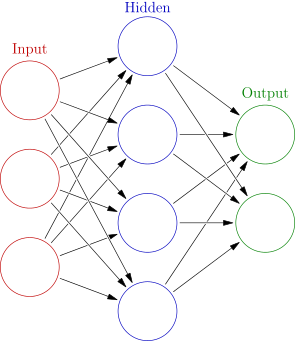
\includegraphics[scale=0.5]{simple_ann.png}
\end{figure}
\\
\\
\noindent
The connections between the neurons from one layer to the next represent the network's weights, each weight again usually just a real number. In addition to these weights between layers, each neuron (aside from the input layer) has an associated bias, once again usually just a real number. Taken across the whole network, these weights and biases form the set of parameters that define the model. They dictate how the activations from neurons in the previous layer should be used to calculate the activations of neurons in the next layer. For instance, let the activations of the neurons in layer \(i\) be given by the vector \(a^{[i]}\), and the weights connecting neurons in layer \(i\) to those in layer \(i+1\) be given by the matrix \(\mathbf{W^{[i+1]}}\). So if the numbers of neurons in layers \(i\) and \(i+1\) respectively are \(n_i\) and \(n_{i+1}\), then \(a^{[i]}\) will have dimension \(n_i \times 1\), and \(\mathbf{W^{[i+1]}}\) dimension \(n_i \times n_{i+1}\)\footnote{Each of the \(n_i\) neurons in layer \(i\) connects to each of the \(n_{i+1}\) neurons in layer \(i+1\), making \({n_i} \times n_{i+1}\) connections in total.}. Then the activations for the neurons in layer \(i+1\) are given by:
\[a^{[i+1]} = f_{i+1}(\mathbf{{W^{[i+1]}}^{\top}}a^{[i]} + b^{[i+1]}) \]
where:
\begin{itemize}
  \item \(b^{[i+1]}\) is the vector of biases for the neurons in layer \(i+1\) (so of dimension \(n_{i+1} \times 1\)). 
  \item \(f_{i+1}\) is the activation function for layer \(i+1\), that applies element-wise to the vector on which it operates, and hence returns a vector. The choice of activation functions is part of the design of the network.   
\end{itemize}
This process is repeated, with activations from the input layer feeding into activations of the first hidden layer; activations from this hidden layer feeding into the next hidden layer; etc until the final activations in the output layer are produced. Note that while \textbf{Figure \ref{fig:simple_ann}} above showed only one hidden layer between input and output, in practice there can be arbitrarily many hidden layers - each taking as input the activations from their previous layer, and sending their own activations as output to the next layer. The choice of the numbers of hidden layers, and the numbers of neurons in each of these layers is again part of the design of the network. 
\\
\\
\noindent
Such networks are called fully-connected networks, and theirs layers with every neuron connecting to every neuron in the next layer are called \textit{fully-connected} or \textit{dense} layers.   

\subsubsection{Activation Functions}
The activation functions are usually chosen to be non-linear - since otherwise, composing several layers of neuron activations reduces to taking a linear function of the original input neurons and the network itself simply becomes a linear function. To see this, let \(f(x) = x\) be the linear activation function used throughout the network. Then if layer \(0\) is the input layer, the activations of layer \(1\) are:
\[a^{[1]} = f(\mathbf{{W^{[1]}}^{\top}}a^{[0]} + b^{[1]}) = \mathbf{{W^{[1]}}^{\top}}a^{[0]} + b^{[1]}\]
And the activations for layer \(2\) are:
\begin{align}
a^{[2]} &= f(\mathbf{{W^{[2]}}^{\top}}a^{[1]} + b^{[2]})  \\
      &= \mathbf{{W^{[2]}}^{\top}}a^{[1]} + b^{[2]} \\
      &= \mathbf{{W^{[2]}}^{\top}}(\mathbf{{W^{[1]}}^{\top}}a^{[0]} + b^{[1]}) + b^{[2]} \\
      &= \mathbf{(W^{[1]}W^{[2]})^{\top}}a^{[0]} + \mathbf{{W^{[2]}}^{\top}}b^{[1]} + b^{[2]} \\
      &= \mathbf{W'^{\top}}a^{[0]} + b' 
\end{align}
where:
\begin{itemize}
  \item \(\mathbf{W'} = \mathbf{W^{[1]}W^{[2]}}\)  is an \({n_0}\times{n_2}\) matrix
  \item \(b' = \mathbf{{W^{[2]}}^{\top}}b^{[1]} + b^{[2]}\) is an \({n_2}\times{1}\) vector
  \item Equation \((4)\) uses the matrix transpose rule \((AB)^{\top} = B^{\top}A^{\top}\)
\end{itemize}
Hence both \(a^{[1]}\) and \(a^{[2]}\) are linear functions of \(a^{[0]}\). This argument can be repeated to any number of hidden layers, and so the output of the whole network (regardless of its size) is simply a linear function of the input. This is undesirable since such a network cannot learn more complicated, non-linear features of the data. Training the network is effectively equivalent to just performing linear regression.
\\
\\
\noindent
Therefore non-linear activation functions are usually preferred. In this project we have used the following activation functions, in line with standard practice for image classification [ref e.g. VGG16].
\\
\\
\noindent
\textbf{ReLU}
\\
\noindent
The Rectified Linear Unit (ReLU) is a scalar activation function that takes a linear function of its argument above a certain threshold \(m\), and is constant otherwise:
\[f(x) = max\{x,m\} \] 
Note that \(m\) is a hyperparameter, specified in advance of training, rather than learning during it. Typically it is just set to 0 - as otherwise this implies some sort of prior knowledge about the scale of the "pre-activation" values \(\mathbf{{W^{[i+1]}}^{\top}}a^{[i]} + b^{[i+1]} \) for all the various layers and neurons in the network (since \(m\) could theoretically be set on a neuron-by-neuron basis). This would be difficult to justify, especially when adjusting the level of these pre-activation values is already handled by the bias term \(b^{[i+1]}\), a parameter that is learned during training.  
\\
\\
\noindent
This activation function introduces a non-linearity at the point \(x=m\), since its slope jumps from 0 to 1 as x increases beyond \(m\). While the function is linear above \(m\), this non-linearity at \(m\) has proven sufficient in practice to obtain good results with ANN's.
\\
\\
\noindent
\textbf{Softmax}
\\
\noindent
The Softmax can be regarded as a vector-to-vector function, that takes as input a vector \(v\), of length (say) \(n\), and produces an output vector \(w\) with the same length as \(v\). The \(j^{th}\) component of \(w\) is given by:
\[w_j = f(v)_j = \dfrac{e^{v_j}}{\sum_{k=1}^n e^{v_k}} \] 
where \(v_j\) is the \(j^{th}\) component of \(v\). Since the Softmax involves exponentiation, it is clearly a non-linear function of its inputs, as desired. Now \({e^x}\geq0 \ \forall \ x \in \mathbb{R} \), so we have \(w_j\geq0\). And, by definition:
\begin{align*}
\sum_{j=1}^n w_j &= \sum_{j=1}^n \dfrac{e^{v_j}}{\sum_{k=1}^n e^{v_k}} \\
&= \dfrac{\sum_{j=1}^n e^{v_j}}{\sum_{k=1}^n e^{v_k}} \\
&= 1 
\end{align*}
Hence \(w_j \in [0,1] \ \forall \ j=1, \ldots,n\) and so \(w\) represents a probability distribution over the set of values \(1, \ldots,n\). This is true regardless of the scale or values of the input \(v\).  
\\
\\
\noindent
This is extremely useful for classification, since we can set the final layer of our ANN to have the same number of neurons as numbers of classes, and let it use the Softmax activation function. Then each neuron would correspond to one of the \(w_j\) above, and the activations across the whole output layer would form a probability distribution over the set of classes. The network then provides a means to go from, say, an image to predicted probabilities of which class        the image belongs to. 
\\
\\
\noindent
More concretely, for our purposes we set the final layer to have 2 neurons - corresponding to normal or abnormal respectively.
\\
\\
\noindent
\textbf{Sigmoid}
\\
\noindent
The sigmoid activation is simply a one-dimensional version of Softmax:
\[ \sigma(x) = \dfrac{e^x}{1+e^x}\]
As with the Softmax, it outputs values in the interval \([0,1]\), which can be thought of as a probability. Sigmoids are often used to provide a soft form of "gating" for a signal, namely the activations from the previous layer in a neural network. Whereas a hard version of gating can only multiply the signal by 1 (to allow all of it through) or 0 (to prevent it entirely), the sigmoid function can vary smoothly between these two extremes. This allows the signal to progress, but dampened by by the factor \(\sigma\), with the extent of dampening required able to be learned during training.  
\newpage
\subsection{Training}
After choosing the structure of the ANN - i.e. the numbers of layers, numbers of neurons, and activation functions for each layer/neuron - it remains to train the network. The act of training the network boils down to setting appropriate values for all the weights and biases across the whole network. While this could be done by hand - this would be very difficult and, for larger networks, the numbers of weights and biases can be several million and hence infeasible to set by hand anyway. Instead, the weights\footnote{We'll use "weights" as a shorthand for "weights and biases" - i.e. the set of model parameters - except where a distinction between the two is necessary.} are initialised to random values and then automatically updated through a process called \textit{Backpropagation}. This involves the following steps:
\begin{itemize}
  \item \textbf{Forward Pass:} data items are input into the network (via the input layer). The activations of each of the subsequent layers are then calculated based on this input, up to the final output layer. Then (since our problem is supervised learning) the output is compared to known, true label for the given data item. This comparison is quantified by a loss function, some chosen function that measures how close the prediction is to the true label.   
  \item \textbf{Backward Pass:} Since the value of the loss function depends on the network's weights (via the predicted label), the gradient of the loss function with respect to each of the weights can be calculated. These gradients then tell us how to adjust (in what direction, by how much) each of the weights in order to reduce the loss - and hence make the prediction closer to the true label.
  \item \textbf{Weight Update:} It remains to make these changes to the weights. Typically we only make a small change vs that indicated by the gradient - since the gradients themselves will be subject to a lot of random variation from data item-to-data item. So making the full change will result in noisy, erratic weight changes, and hence also erratic changes in the predictions with each weight update. So instead we multiply all of the gradients by some small number \(\eta\) (e.g. \(\eta\approx0.001\)) called the \textit{learning rate}. This has the effect of slowing down the weight updates, and hence allowing a more gradual progression towards a minimum of the loss function. 
\end{itemize}
There are in fact a number of different training algorithms, which vary in the details, but all of the ones we consider follow this basic pattern.

\subsubsection{Loss Functions}
As mentioned, loss functions are used to measure how far away predicted labels, generated by the network, are from the true label. Predictions that are "close" to the true label should have a smaller loss than predictions that are further away. For any item of data, both the activations in the network's input layer, and the item's true label are fixed. So the only aspect of a given network that we are free to vary are its weights, since these determine how the prediction is generated for an item of data. Therefore we can regard the loss as a function of the network's weights - and the goal of training is to set these weights so as to minimise the expected loss over a collection of data items.
\\
\\
\noindent
The loss function we have used in this project is the cross-entropy loss, again in line with standard practice for image classification.
\\
\\
\noindent
\textbf{Cross-Entropy Loss}
\\
\noindent
The cross-entropy loss assumes that the true label \(y\) (i.e. the class to which the data item belongs) is coded as a "one-hot" vector. If there are \(n\) classes, \(y\) is a vector of length \(n\), with each component corresponding to one of these classes. All components of \(y\) are set to 0, except for the component corresponding the class to which \(y\) belongs - which is set to 1. 
\\
\\
\noindent
So for our x-ray data we code the two classes as follows:
\begin{itemize}
  \item Normal: \([1, 0]\)   
  \item Abnormal: \([0, 1]\)   
\end{itemize}
The predicted label $\hat{y}$, per the Softmax activation function in the output layer, represents a probability distribution over the \(n\) classes - and so has the same dimension as \(y\).
\\
\\
\noindent
The cross-entropy loss is then given by:
\[L(y,\hat{y}) = - \sum_{j=1}^n y_jlog(\hat{y_j})   \]
Note that since \(y\) has all components 0, except for a 1 corresponding to the true label, the loss above reduces to taking the logarithm of the predicted probability of the true label. The sign of the logarithm is negated, so that smaller probabilties, which would give larger negative values of log, give larger positive loss values. The loss is therefore monotonically decreasing with the predicted probability of the true label - which is as desired, since predicting a high probability for the true label should have a smaller loss than predicting a lower probability.  

\subsubsection{Backward Pass}
After performaing a forward pass and calculating the loss for a given data item, we now calculate the gradients of the loss with respect to all the weights and activations in the network. This is called a backward pass since the gradients in one layer depend on those in the subsequent layer. Hence the process starts with calculating gradients in the output layer, then the gradients for the previous layer, and so on all the way back through the whole network. While the weight update step of the Backpropagation algorithm only uses the gradients of the weights, these gradients themselves depend on the gradients of the activations of the neurons which depend on these weights. Thus the backward pass involves calculating the gradients of activations, even though these are not strictly used in the weight update step. 
\\
\\
\noindent
Using the cross-entropy loss function, for a classification task as described above, we can calculate the gradient of the loss with respect to $\hat{y_j}$ (considering \(y_j\) as a fixed constant):
\begin{align*}
\dfrac{\partial  L}{\partial \hat{y_j}} &= \dfrac{\partial }{\partial \hat{y_j}}(- \sum_{j=1}^n y_jlog(\hat{y_j})) \\
&= \dfrac{\partial }{\partial \hat{y_j}}(-y_jlog(\hat{y_j})) \\
&= -\dfrac{y_j}{\hat{y_j}}
\end{align*}
Recall that $\hat{y_j}$ is the activation of the \(j^{th}\) neuron in the output layer. Which itself is a derived from the weights \(\mathbf{W}\) and biases \(b\) in the output layer, and the activations from the previous layer (layer \(l\), say) \(a^{[l]}\), fed through the Softmax function:
\[ z = \mathbf{W^{\top}}a^{[l]} + b\]   
\[ \hat{y_j} = \dfrac{e^{z_j}}{\sum_{k=1}^n e^{z_k}} \]
And so, by the quotient rule:
\begin{align*}
\dfrac{\partial  \hat{y_j}}{\partial z_j} &= \dfrac{e^{z_j}(\sum_{k \neq j}e^{z_k}+e^{z_j}) - (e^{z_j})^2}{(\sum_{k=1}^n e^{z_k})^2} \\
&= \dfrac{e^{z_j}}{\sum_{k=1}^n e^{z_k}} \dfrac{\sum_{k \neq j}e^{z_k}}{\sum_{k=1}^n e^{z_k}} \\
&= \hat{y_j}(1-\hat{y_j})
\end{align*}
Where the final equality is due to:
\begin{align*}
1-\hat{y_j} &= 1 - \dfrac{e^{z_j}}{\sum_{k=1}^n e^{z_k}} \\
&= \dfrac {\sum_{k=1}^n e^{z_k} - e^{z_j}}{\sum_{k=1}^n e^{z_k}} \\
&= \dfrac {\sum_{k \neq j} e^{z_k}}{\sum_{k=1}^n e^{z_k}}
\end{align*}
Therefore we can apply the chain rule of differentiation to calculate the gradients of the loss with respect to the weights and biases in the output layer as follows:
\begin{align*}
\dfrac{\partial L}{\partial z_j} &= \dfrac{\partial L}{\partial \hat{y_j}} \dfrac{\partial \hat{y_j}}{\partial z_j} \\
&= \dfrac {y_j}{\hat{y_j}} \hat{y_j}(1-\hat{y_j}) \\
&= y_j(1-\hat{y_j})
\end{align*}
Now if layer \(l\) has \(n_l\) neurons:
\[ z_j = \sum_{i=1}^{n_l} w_{i,j}a^{[l]}_i + b_j\]
So:
\[ \dfrac{\partial z_j}{\partial w_{i,j}} = a^{[l]}_i \]
\[ \dfrac{\partial z_j}{\partial b_j} = 1 \]
And we have:
\begin{align*}
\dfrac{\partial L}{\partial w_{i,j}} &= \dfrac{\partial L}{\partial z_j}\dfrac{\partial z_j}{\partial w_{i,j}} \\
&= y_j(1-\hat{y_j})a^{[l]}_i
\end{align*}
\begin{align*}
\dfrac{\partial L}{\partial b_j} &= \dfrac{\partial L}{\partial z_j}\dfrac{\partial z_j}{\partial b_j} \\
&= y_j(1-\hat{y_j})
\end{align*}
where \(w_{i,j}\) is an element from \(j^{th}\) column of the weight matrix \(\mathbf{W}\), and \(b_j\) the bias of the \(j^{th}\) neuron in the output layer. 
\\
\\
\noindent
We can also obtain similar formulas for the gradients of the loss with respect to the activations in layer \(l\). Since each neuron in this layer connects to all neurons in the output layer, a given activation \(a^{[l]}_i\) will appear in the formula (as shown above) for all \(z_j\), \(j=1,\ldots,n\). And each of the \(z_j\) appear additively in the loss function via $\hat{y_j}$. Therefore we have:
\[ \dfrac{\partial z_j}{\partial a^{[l]}_i} = w_{i,j}\]
\begin{align*}
\dfrac{\partial L}{\partial a^{[l]}_i} &= \sum_{j=1}^{n} \dfrac{\partial L}{\partial z_j}\dfrac{\partial z_j}{\partial a^{[l]}_i} \\
&= \sum_{j=1}^{n} y_j(1-\hat{y_j})w_{i,j}
\end{align*}
But these activations \(a^{[l]}\) themselves depend on the weights and biases in layer \(l\), and so we can extend the chain rule further to calculate the gradient of the loss with respect to these as well. And we can repeat this process for the activations, weights and biases, in layers \({l-1}, {l-2}, \ldots \) etc all the way back through the entire network.   

\subsubsection{Weight Update}
The gradients calculated in the backward pass above give the change in weight to make, in order to increase the loss function. Since we aim to decrease our loss function, we subtract the gradients from the current values of all the weights. However, as mentioned, we first multiply the gradients by a hyperparameter \(\eta\), called the learning rate, in order to avoid large, erratic changes in weights (and hence predictions) after each weight update. That is, for a weight (or bias) \(w\) in the network, with gradient \(\dfrac{\partial L}{\partial w}\) we apply the following update:
\[ w = w - \eta \dfrac{\partial L}{\partial w} \]

\subsubsection{Optimisers}
The following algorithms are all variations on the general theme of Backpropagation described above. That is, they all concern how to set the weights in order to minimise the loss function, based on the gradients of the loss function (hence the algorithms are called "optimisers"). 
\\
\\
\noindent
\textbf{Gradient Descent}
\\
\noindent
This involves performing a forward pass, calculating the activations and the loss, then performing a backward pass, calculating the gradients of all the weights, for every item of data in the training set. The gradients of each weight are then averaged across the entire set of training data, before performing the weight update using these average values for each weight. That is, for a weight \(w\) let  \({\dfrac{\partial L}{\partial w}}_i\) be its gradient after  forward and backward passes with the \(i^{th}\) element of the training set as input to the network. Then if there are \(n\) items of data in the training set, perform the following weight update:
\[ w = w - \dfrac{\eta}{n}\sum_{i=1}^{n} {\dfrac{\partial L}{\partial w}}_i \]
That is, we have to perform a forward pass and backward pass for every item in the training set, and keep track of all associated gradients, before making a single weight update. This can be both slow and consume a lot of memory (consider a large network with millions of weights, and a large training set with millions of items). Note this process will often be repeated, with training involving hundreds or thousands of weight updates.
\\
\\
\noindent
\textbf{Stochastic Gradient Descent}
\\
\noindent
Stochastic gradient descent (SGD) aims to speed things up by dividing the training set up into batches of a certain size (say, 128). Each data item in the training set is assigned randomly (hence "stochastic") without replacement to each of the batches. Then the weight updates are performed after calculating and averaging the gradients for each item in a batch. That is, if the batches are of size \(m\), for a given weight we make the following update:
\[ w = w - \dfrac{\eta}{m}\sum_{i=1}^{m} {\dfrac{\partial L}{\partial w}}_i \]
where \({\dfrac{\partial L}{\partial w}}_i\) is the gradient of \(w\) for the \(i^{th}\) item in the batch. An \textit{epoch} is then defined as a pass through the full set of batches, performing a weight update for each batch. Thus if the training data of size \(n\) is split up into batches of size \(m\), an epoch would involve \( \left \lceil{\dfrac{n}{m}}\right \rceil \)\footnote{\( \left \lceil{x}\right \rceil \) is the smallest integer greater than or equal to \(x\). If \(m\) does not divide into \(n\), the final batch will comprise \((n \mod m)\) items to ensure an epoch covers the entire training set.} weight updates - compared to just one for ordinary Gradient Descent. Training using SGD often involves running for several epochs. The random assignment of the training data into batches is repeated fresh at the start of each epoch.
\\
\\
\noindent
The advantage of SGD is that it is clearly quicker than GD to perform weight updates. While each weight update will be subject to more randomness than in GD, since each update corresponds to a single, random batch rather than the full training set. However, over the course of several hundred or thousand weight updates, involving many epochs or passes over the whole training set, this should average out to give comparable results to GD. 
\\
\\
\noindent
\textbf{RMSProp}
\\
\noindent
One of the issues with GD and SGD is that the learning rate \(\eta\) is a global hyperparameter that is fixed for all the weights in the network, and for all weight update iterations. However in practice, some weights in the network will require larger or smaller updates than others and, over the course of training, the weight updates will usually need to get smaller and smaller for successive iterations, as we approach a minimum of the loss function. RMSProp aims to solve these problems by effectively allowing the learning rate to vary during training and for each weight.
\\
\\
\noindent
Let \(w_t\) be a weight in the network, and let \(g_t = {\dfrac{\partial L}{\partial w}}_t\) be its gradient, at iteration \(t\). Then over all iterations we keep an exponential moving average of the square of these gradients:
\[ v_t = \alpha g_t^2 + (1-\alpha)v_{t-1} \]
where the base case is \(v_0 = 0\), and \( \alpha \in [0,1]\) is a chosen hyperparameter that determines the extent to which (squared) gradients from past iterations affect the value of \(v_{t+1}\). Note that an iteration can refer either to a full pass over the whole training set, as in GD, or over a batch, as in SGD. Although in practice we will use it in conjunction with SGD, since it inherits the benefits mentioned above. So the "gradient" \(g_t\) above would in fact be the average of the gradients for the weight across a batch. The weight update for the given iteration is then:
\[ \delta_t  = \dfrac{\eta}{\sqrt{v_t} + \epsilon} g_t \]
\[ w_{t+1} = w_t - \delta_t \]
where \(\eta\) is the (global) learning rate, and \(\epsilon\) is some small number (e.g. \(\epsilon=10^{-6}\)) added to avoid division by 0. The \(\dfrac{\eta}{\sqrt{v_t} + \epsilon}\) term now means that the learning rate \(\eta\) is dampened by the factor \(\sqrt{v_t} + \epsilon\), which varies for each training iteration and for each weight in the network. So for a weight that had larger gradients in previous iterations, so a larger \(v_t\), the effective learning rate will be smaller. Hence its subsequent weight updates get smaller as training progresses - slowing them down compared to weights with smaller gradients and weight updates at earlier iterations. This is desired, since weights that have seen large changes over training are more likely to be closer to the loss function minimum on which they are converging, and so should progress more slowly towards it (to avoid overshooting it, or other erratic behaviour).
\\
\\
\noindent
\textbf{Adam}
\\
\noindent
The Adam ("Adaptive Momentum") optimiser is a variation on RMSProp that takes account of momentum in the gradients from previous epochs. That is, large gradients on several previous iterations should not be ignored if the current gradient (by chance) happens to be very low, or vice versa. The momentum effect produces smoother and less erratic weight updates than RMSProp. To this end, Adam maintains an exponential moving average of the gradient \(g_t\), as well as the squared gradient of RMSProp:
\[ m_t = \beta g_t + (1-\beta)m_{t-1} \]
Again the base case is \(m_0=0\), and \( \beta \in [0,1]\) is another hyperparameter that determines to what extent past gradients are taken credit for. The weight update is then:
\[ \delta_t  = \dfrac{\eta}{\sqrt{v_t} + \epsilon} m_t \]
\[ w_{t+1} = w_t - \delta_t \]
where \(v_t\), \(\eta\) and \(\epsilon\) are defined as in RMSProp. This has the same benefits as RMSProp of dampening the learning rate \(\eta\) during training, but the weight update uses the smoothed \(m_t\) rather than the raw \(g_t\) at each iteration. 

\subsubsection{Weight Initialisation}
Prior to training, all weights and biases in the network need to be initialised to some reasonable values. If they were all simply set to 0, the activations of all neurons in the network, and hence all the gradients would just be 0 too. Therefore the weight update step would leave all weights unchanged, and "training" would accomplish nothing. Instead weights are usually initialised to random values. This effectively sets the initial position on the (multidimensional) loss surface, considering the loss as a function of the network's weights. Training then proceeds from this initial position towards a minimum of this loss function. Therefore performing different instances of training (even on the same data) ab-initio can lead to different solutions, since each instance will have a different starting position on the loss surface, and hence converge toward different minima. However the choice of optimiser should help mitigate this problem, e.g. by avoiding shallow local minima, and progressing towards deeper, more global minima\footnote{Of course, the loss surface is usually very high dimensional, and depends on the training data. So it is hard to have any clarity over its precise form or nature. In any case, it is often not necessary for the task at hand - networks are typically trained until they achieve some desired level of performance, regardless of whether this represents a true global minimum or not.}. For this project we have used the following weight initialisation scheme, since that is the default in the software (Keras) we used to train our models.
\\
\\
\noindent
\textbf{Glorot Uniform}
\\
\noindent
This initialisation scheme was introduced by Xavier Glorot and Yoshua Bengio in 2010 \cite{glorot_uniform}. It initialises biases to 0, and the weights \(w_{i,j}\) in each layer randomly according to the distribution:
\[ w_{i,j} \sim U[-\dfrac{1}{\sqrt{n}}, \dfrac{1}{\sqrt{n}}] \]
where \(U[a,b]\) is the continuous random uniform distribution over the interval \([a,b]\), and \(n\) is the number of neurons in the previous layer.
\\
\\
\noindent
In fact, examining the Keras source code \cite{keras_source}, Glorot Uniform is implemented slightly differently to how it was introduced by Glorot \& Bengio. Biases are still initialised to 0. However weights are drawn randomly from \(U[-limit,limit]\) with \(limit = \sqrt{\dfrac{6}{fan\_in + fan\_out}}\) where \(fan\_in\) is the number of input neurons to the weight tensor, and \(fan\_out\) the number of output neurons. In our terms, if \(\mathbf{W}\) is the \(n_i \times n_{i+1}\) matrix of weights connecting layers \(i\) and \(i+1\), then each element \(w\) of \(\mathbf{W}\) will be initialised as above, with \(fan\_in = n_i\) and \(fan\_out = n_{i+1}\).  


\subsubsection{Regularisation}
Regularisation is used to prevent overfitting by neural networks - i.e. the fact that, while the network may perform well on the data on which it was trained, its performance on another set of data is poor. This usually occurs because, while training, the network captures too much of the random noise present in the training data, and therefore does not transfer well to another data set where that noise is not present (instead having its own random noise). So regularisation aims to ensure that training leads networks to capture genuine features of the data that will be present in other data sets, rather than that random noise. We describe some regularisation techniques below: 
\\
\\
\noindent
\textbf{Dropout}
\\
\noindent
Dropout was introduced by Srivastava et al in 2014 \cite{dropout_paper}. The idea is, for a given network layer, to randomly remove some neurons from that layer. At each training iteration, e.g. for each batch in SGD, each neuron and its associated weights and biases are retained in the network with some chosen probability \(p\), and removed with probability \(1-p\). This random selection is performed fresh for each iteration, so that each iteration effectively uses a slightly different network architecture. That means that the paths for information to travel through the network - the sequence of neurons and connections between them - vary. This introduces redundancy in that the same genuine features of the data are learned by several routes through the network, since the available routes change with each iteration. This reduces the likelihood that parts of the network just start capturing noise, as for any given iteration those parts of the network may or may not be present. Further, for any given epoch, each neuron will only see an expected fraction \(p\) batches of training data, and is therefore exposed to less noise in the data. So the neuron's weights will be less likely to capture noise.        
\\
\\
\noindent
Dropout also reduces the effective capacity of the network layer at each iteration by the factor \(p\). A layer with 10 neurons and dropout probability 70\%, would only use an expected 7 neurons. This reduces the scope of the layer to capture noise in the data, since there are fewer effective parameters. So there is less "room" for the network layer to pick up noise.
\\
\\
\noindent
After training, say when testing the network on a validation set, we revert to the full original network architecture - neurons are no longer dropped out. Instead, a trained weights \(w\) in a given dropout layer are replaced with \(pw\). A forward pass can then be conducted as normal. 

\newpage
\subsection{Convolutional Neural Networks}
Convolutional neural networks (CNN's) are a variant of artificial neural networks described above, that are often used for image processing tasks such as classification. They are organised as a sequence of "convolution" layers, where the first layer operates directly on an image to produce a representation of it comprised of various low-level features, such as edges or patches of light or dark etc. The next layer then operates on this representation, producing another representation that captures slightly higher-level features, based on compostions of the low-level features from the first layer. This process is repeated for a chosen number of layers, with each layer outputting a representation based on the one from the previous layer. The final output from the sequence of convolution layers is then some representation of the original image built up from the low- and mid-level features from past layers. This final representation can then be used for the task at hand - for instance fed through a fully-connected layer, into a Softmax output layer for classification.     
\\
\\
\noindent
The strength of CNN's is that the representations they produce can pick up features regardless of where they appear in the image. So if a representation captures the shape and colour patterns of eyes (say), it will "recognise" eyes that appear at any position in the image. This property is called \textit{translational invariance}. By contrast, if the original image was fed through a sequence of fully-connected layers, different weights in the network would correspond to different positions in the image. So that any feature learned by some subset of the weights would only be recognised if it appeared at the corresponding position in the image.
\\
\\
\noindent
Another strength is that the numbers of weights in convolution layers are not tied to the size of the image, whereas a fully-connected layer would be. Therefore the number of weights in a given layer can be significantly smaller than for a corresponding fully-connected layer. This makes training the network easier, since there are fewer weights to set. For instance, consider a \(100 \times 100\) image fully-connected to a hidden layer of 10 neurons - this would have \(100 \times 100 \times 10 = 100,000\) weights. Meanwhile a convolution layer might have, say, 30 \(3 \times 3\) filters - making \(30 \times 3 \times 3 = 270\) weights. This independence from the size of images means that previously-trained CNN's can be used on different sets of images (potentially of entirely different dimensions) from those it was originally trained on, and still identify the same features in both sets of images. This makes CNN's very convenient for transferring from one image processing task to another - so-called \textit{transfer learning}. 

\subsubsection{Image Representation}
Throughout this section, we represent an image as either a 2D or 3D grid of pixel values, where the height and width of the image are the first two dimensions, and the channels of the image are the third dimesion. For greyscale images, there is only one channel, so we regard the image as being 2D. For colour images coded as RGB (say), there are three channels (red, green, blue) so we regard the image as 3D with depth 3.  

\subsubsection{Convolution Layers}
A convolution layer represents a collection of \textit{filters} of a chosen dimension - say, \(3 \times 3\). Each element of a filter is a real number, and is one of the weights of the convolution layer to be learned during training. The filter will operate on all channels of its input image or representation (from previous convolution layers). So a \(3 \times 3\) filter working on an RGB image will have \(3 \times 3 \times 3 = 27\) weights, since the image has 3 channels. The output of each filter in a convolution layer is passed to the next convolution layer as a separate channels - so that if the first layer has (say) 32 filters, the filters in the next layer will have a depth of 32. If the next layer uses \(5 \times 5\) filters, each one will have \(5 \times 5 \times 32 = 800\) weights\footnote{In fact, each filter has a single associated bias term (regardless of depth), so the filters mentioned would have 28 and 801 parameters respectively.}.    
\\
\\
\noindent
Each filter performs a convolution operation between its input and its weights. For a one-channel input, this is defined as follows. Let $\begin{bmatrix}w_{1,1} & w_{1,2}\\ w_{2,1} & w_{2,2}\end{bmatrix}$ be a \(2 \times 2\) filter and \(b\) be its associated bias. Let $\begin{bmatrix}p_{1,1} & p_{1,2}\\ p_{2,1} & p_{2,2}\end{bmatrix}$ be the values for some contiguous \(2 \times 2\) region of the input.
The convolution is then:
\[ z = \sum_{i=1}^2 \sum_{j=1}^2 w_{i,j}p_{i,j} + b \]  
\[ a = f(z) \]
That is, we take the element-wise product of the corresponding weights and input values, then sum all of them. The function \(f\) is some chosen activation function (e.g. ReLU). For a multiple-channel input, the filter and input will be 3-dimensional, and the operation would instead apply to a contiguous 3D volume of the input. For instance, if the input were an RBG image and the filter were now of dimension \(n \times n\), the convolution would look like:
\[ z = \sum_{i=1}^n \sum_{j=1}^n \sum_{k=1}^3 w_{i,j,k}p_{i,j,k} + b \]
\[ a = f(z) \]
This convolution operation is repeated multiple times, over many positions in the input. It first applies at the top-left corner of the input - for the one-channel \(2 \times 2\) filter, say this is $\begin{bmatrix}p_{1,1} & p_{1,2}\\ p_{2,1} & p_{2,2}\end{bmatrix}$ - with result \(a_{1,1}\). Then the filter will shift to the right some chosen number of columns, called the \textit{stride}, and perform the convolution operation again on this new region of the input - with result \(a_{1,2}\). However for convolution layers, the stride is usually just set to 1 - so that for our \(2 \times 2\) filter, the second position is $\begin{bmatrix}p_{1,2} & p_{1,3}\\ p_{2,2} & p_{2,3}\end{bmatrix}$. This continues on until the right-hand edge of the input is reached, at which point the filter moves down some number of rows, again given by the stride. So if the input has width \(w\), the \(2 \times 2\) filter with stride 1 would now apply to the region $\begin{bmatrix}p_{2,w-1} & p_{2,w}\\ p_{3,w-1} & p_{3,w}\end{bmatrix}$ - with result \(a_{2,w-1}\). Then filter would then move from right-to-left over this new row, before moving down to the next row. This continues until the filter has performed a sweep of the whole input, applying the convolution to the corresponding input values at each position. 
\\
\\
\noindent
This produces a set of values $\begin{bmatrix}a_{1,1} & a_{1,2} & \dots \\ a_{2,1} & a_{2,2} & \dots \\ \vdots & \vdots & \ddots \end{bmatrix}$ which we call the representation of the input, produced by the filter. These are organised spatially into a 2D grid based on the position on the input to which they correspond - i.e. \(a_{1,1}\) corresponds the to top-left position etc. If the convolution layer consists of several filters, each one will produce one of these 2D grids, and we stack the set of these grids into a 3D volume - with each grid considered a separate channel. This 3D volume is then the layer's output representation, on which the next convolution layer will operate.         
\\
\\
\noindent
The set of weights that consitutes a filter are kept the same for every convolution operation at every position on the input. This explains the translational invariance property, since the filter will pick up the same feature, wherever in the input it appears. 
\\
\\
\noindent
Filters are usually chosen to be square - i.e. to have the same height and width - so as not to bias them in advance towards picking up features of one orientation over another. A filter that was taller than it was wide would be more likely to pick up vertically-oriented features. Instead we would rather the filter to be initially "neutral" in that regard, and learn to pick up vertical features during training if appropriate. 
\\
\\
\noindent
Filters are also usually chosen to have odd height and width, rather than even (e.g. \(3 \times 3\) rather than \(2 \times 2\)). This is so that the filter has a well-defined center, and we can think of the position of the filter on the input as that corresponding to the central weight in the filter. So if a \(3 \times 3\) (one-channel) filter covers the input region $\begin{bmatrix}p_{x-1,y-1} & p_{x,y-1} & p_{x+1,y-1} \\ p_{x-1,y} & p_{x,y} & p_{x+1,y} \\ p_{x-1,y+1} & p_{x,y+1} & p_{x+1,y+1} \end{bmatrix}$, we can call the result of the convolution operation \(a_{x,y}\). This produces a convenient alignment between the input and the representation produced from it, and in the absence of a compelling reason for an even-dimension filter we might as well use it.     

\subsubsection{Padding}
Padding allows for the representation produced from an input to have the same height and width as the input. Note that if we position a \(3 \times 3\) filter in the top-left corner of the input, its central weight would not correspond to the top-left pixel\footnote{We'll use "pixel" loosely to mean either one cell in the original image (thought of as a 2D or 3D grid), or one cell in the representation produced by a convolution layer.} - instead to the pixel down-and-to-the-right by one. And similar when the filter is postioned in the top-right, bottom-left etc. This means that there would be no positions in the output representation corresponding to the top or bottom rows of the input, nor the rightmost or leftmost columns. So an \(h \times w \) input would reduce to a \(h-2 \times w-2 \) representation. Padding inserts values of 0 around the edge of the input - effectively increasing its dimension to \(h+2 \times w+2 \) - so that the top-left position can correspond to the actual top-left pixel of the input. So the resulting output representation would then be \(h \times w \) as desired. The amount of padding layers will depend on the dimension of the filter - a \(5 \times 5\) filter would have 2 such padding layers, and so on.

\subsubsection{Pooling Layers}
Pooling layers are used to reduce the size of representations, while still retaining their key features. This is also called downsampling. It is useful when using the final representation produced by a sequence of convolution layers for further tasks. For example, feeding it through a fully-connected layer in order to perform classification. If we had used padding, the final representation would have the same height and width as the original image, and potentially many more channels depending on the number of filters used in the final convolution layer. The fully-connected layer would therefore be extremely large, and have a very large number of parameters.   
\\
\\
\noindent
Moreover, downsampling in between convolution layers allows the subsequent layer to more easily capture spatial combinations of the features created in the previous layer. In particular doing so using smaller filter sizes (and hence fewer trainable weights) than would otherwise be necessary. That is, if the key features of an \(h \times w\) representation are compressed into a smaller, say, \(\dfrac{h}{2} \times \dfrac{w}{2}\) representation - an \(n \times n\) filter would now be able to capture combinations of features that were further than \(n\) pixels apart in the original representation, if they are now within \(n\) pixels in the new representation. As this process continues over several layers, with representations getting progressively smaller, the convolution operations are better able to progress from isolated low-level features of the original image, to mid- then high-level combinations of such features across the whole image.
\\
\\
\noindent
The pooling layers themselves again involve a window of some chosen dimension, again usually square, and stride. However the stride is now usually (though not necesarily) set equal to the height/width of the window. The window will move across the input in the same manner as the filter in a convolution layer - in increments of the chosen stride. However instead of performing the convolution operation, it will instead perform some aggregation of the pixel values corresponding to its position on the input. Typically taking either the maximum or the sum of these values. This will then form the value for one cell in the represention produced by the pooling layer. Since it is simply aggregating pixel values, the pooling layer has no associated weights, and so does not need to be trained. Also, the pooling layer only operates on the two spatial dimensions - so for a multi-channel input, it will operate on each channel separately. The representation produced by the pooling layer will therefore have the same number of channels as its input, but a smaller height and width.
\\
\\
\noindent
Consider a \(2 \times 2\) window with stride 2. This will start in the top-left corner of the input and produce a single value. Then it will move two columns to the right to produce the next value. This means that if the input was dimension \(h \times w\), the representation from the pooling layer will have dimension \(\dfrac{h}{2} \times \dfrac{w}{2}\). Taking the max or summing the pixel values means that the key information is retained from the input representation - since large pixel values correspond to the presence of the feature that the filter (whose convolution operation produced the pixel values) has been trained to capture. 

\subsubsection{Prediction}
In the context of image classification, the predictions we make from a convolution net are a probability distribution over a given set of classes. This is done using a Softmax as described above. The network itself will comprise of a sequence of convolution and pooling layers that produce some final representation of the input image. While this final representation is typcially a 3D volume, we introduce a "flatten" layer that treats each cell in this 3D volume as a neuron. So if the final output of the convolution layers is, say, a \(10 \times 10 \times 5\) 3D volume, after flattening we get a 500 neuron layer. This flatten layer is then connected to an intermediate, fully-connected hidden layer, which is then connected to the output Softmax layer. So the connections from the flatten layer to the intermediate hidden layer form another set of of weights (and biases) to be learned, as do those from the hidden to the output layer. Of course, we could introduce further hidden layers prior to the output layer, if necessary. In effect, we can treat the flatten layer as the input layer of a separate, fully-connected network. We can think of this as the "head" of the convolutional network, while the preceding convolution and pooling layers form its convolutional "base".
\\
\\
\noindent
This separation allows for transfer learning as described above. We can replace simply the head, while retaining the convolutional base - both its structure, and the weights and biases of its filters. This means that the convolutinal base will still pick out the same features, combinations of features etc, in the same way when applied to a new set of images. We can then use these as inputs for the new network head, which may need to have a different design than the head with which the convolational base was originally trained with. For instance, if our new image classification task involves a new (smaller or larger) set of classes than those originally trained on - the output Softmax layer would have to change to match the new number of classes.
\\
\\
\noindent
One slight downside of using a fully-connected head, is that the size of the flatten input layer is dependant on the size of the input image - say all our filters use padding, and we have two pooling layers of window size \(2 \times 2\) with stride 2. Then the final representation will have one quarter the height and one quarter the width of the original image. This means, if we're performing training over a set of images, each image in the set must have the same dimension. Otherwise, the flatten layer would vary in size with each image, and so the number of weights between the flatten and hidden layer in the head. 

\subsubsection{Training}
Convolutional networks can be trained in the exactly the same way as for general artificial neural networks described above- that is, by Backpropagation via algorithms such as SGD or Adam. As mentioned, the weights for convolutional layers are the values in the filters. We can perform a backward pass through both the head and convolutional base to calculate the gradients of the loss with respect to the weights and biases in all filters, throughout the whole network. 
\\
\\
\noindent
However in transfer learning, the weights in the convolutional base are often left unchanged. Instead only the weights in the head are trained on the new set of data - they generally can't be reused (even if the head has the same structure) since they will be specific to the set of labels originally trained on. Whereas the convolutional base captures fairly generic features that will have relevance across a range of image processing tasks. 

\newpage
\subsection{Performance Measures}
We now introduce the measures we use to asses the performance of our trained network. While the network is trained using the cross-entropy loss, as described above, we can report other measures that capture other aspects of performance more explicitly e.g. the false positive or false negative rates. Typically we are interested on the performance of the network on an alternative data set to that on which it was trained - a so-called valiation set.   

\subsubsection{Accuracy}
This is probably simplest measure of performance. For each item in the validation set, we have the true label (e.g. normal or abnormal). The network outputs a predicted probability of each class for each data item. So we can let the network's predicted label be the class that has the largest predicted probability. Let the true class label be \(y\) and the predicted label be \(\hat{y}\), and the validation set consist of \(m\) data items. The accuracy is then:
\[ accuracy = \dfrac{1}{m} \sum_{i=1}^m I(y=\hat{y}) \]
where
\[ I(y=\hat{y}) = \begin{cases}
1 \quad \text{if } y=\hat{y}\\
0 \quad \text{otherwise}\\
\end{cases}\]
That is, accuracy simply measures the proportion of correct predictions the network makes on a dataset.

\subsubsection{Confusion Matrix}
The confusion matrix decomposes the correct and incorrect predictions for each class. An example for our two classes \textit{Normal} and \textit{Abnormal} is shown below:
% Create Confusion Matrix - adapted from https://tex.stackexchange.com/questions/20267/how-to-construct-a-confusion-matrix-in-latex/338931. Note: need the multirow package
\begin{figure}[ht]
    \centering
  \caption{Confusion Matrix Example}
    \begin{tabular}{l|l|c|c|c}
    \multicolumn{2}{c}{}&\multicolumn{2}{c}{\textbf{True Label}}&\\
    \cline{3-4}
    \multicolumn{2}{c|}{}&\textbf{Normal}&\textbf{Abnormal}&\multicolumn{1}{c}{\textbf{Total}}\\
    \cline{2-4}
    \multirow{2}{*}{\textbf{Predicted Label}}& \textbf{Normal} & $a$ & $b$ & $a+b$\\
    \cline{2-4}
    & \textbf{Abnormal} & $c$ & $d$ & $c+d$\\
    \cline{2-4}
    \multicolumn{1}{c}{} & \multicolumn{1}{c}{\textbf{Total}} & \multicolumn{1}{c}{$a+c$} & \multicolumn{1}{c}{$b+d$} & \multicolumn{1}{c}{$a+b+c+d$}\\
    \end{tabular}
    \label{fig:confusion_matrix_example}
\end{figure}
% End Confusiom Matrix Code
\\
\\
\noindent
That is, the network predicted \(a\) examples with true label \textit{Normal} as \textit{Normal}, etc. So the accuracy would be \( \dfrac{a+d}{a+b+c+d}\). 
\\
\\
\noindent
Now if we consider \textit{Normal} to be "negative" and \textit{Abnormal} to be "positive", we can define:
\begin{itemize}
  \item \textbf{True Negative Rate} Proportion of true \textit{Normal} labels predicted correctly: \( \dfrac{a}{a+c} \)
  \item \textbf{False Negative Rate} Proportion of true \textit{Abnormal} labels incorrectly predicted as \textit{Normal}: \( \dfrac{b}{b+d} \)
  \item \textbf{True Positive Rate} Proportion of true \textit{Abnormal} labels predicted correctly:  \( \dfrac{d}{b+d} \)
  \item \textbf{False Positive Rate} Proportion of true \textit{Normal} labels incorrectly predicted as \textit{Abnormal}: \( \dfrac{c}{a+c} \)
\end{itemize}

\subsubsection{Cohen's Kappa}
Cohen's Kappa was introduced by Jacob Cohen in 1960 \cite{cohens_kappa}. It is a measure of agreement between two raters - so when applied to a corresponding set of true and predicted labels, it measures the accuracy of the predictions. Its advantage over simple accuracy is that is measures the extent of agreement over and above that which would be expected by chance. This is useful for instance when the class frequencies in the underlying data are naturally skewed. Consider data comprised of two classes, 80\% A and 20\% B - a classifier that simply always predicted A would have 80\% accuracy, but can not be considered a very good classifier. Cohen's Kappa accounts for this underlying skew, and would score the classifier poorly. For the confusion matrix in \textbf{Figure \ref{fig:confusion_matrix_example}} above, it is defined as follows:
\\
\\
\noindent
Let \(p_o = \dfrac{a+d}{a+b+c+d}\) be the observed overall accuracy.
\\
\\
\noindent
Now let \(p_e = p_{normal} + p_{abnormal}\) be the probability of agreement at random, where:
\[p_{normal} = \dfrac{a+b}{a+b+c+d} \ \dfrac{a+c}{a+b+c+d} \]
\[p_{abnormal} = \dfrac{c+d}{a+b+c+d} \ \dfrac{b+d}{a+b+c+d} \]
Cohen's Kappa is then:
\[ \kappa = \dfrac{p_o - p_e}{1-p_e} \]
Cohen's Kappa usually ranges from 0, when the observed accuracy is simply equal to that expected at random (i.e. \(p_o = p_e\)) - to 1, when the observed accuracy is 100\% (i.e. \(p_o=1\)), regardless of the extent of expected random agreement \(p_e\)\footnote{Ignoring the degenerate case \(p_e=1\).}. It can be negative, when the observed accuracy is \textit{below} that expected by chance, but this should be rare in practice.
\subsubsection{ROC Curve}
The ROC curve is a way to illustrate the performance of one or more binary classifiers, allowing for convenient comparison. An example \cite{wiki:ROC_Curve} is shown below:  
\begin{figure}[!ht]
  \centering    
  \caption{Example of a ROC Curve plot}
  \label{fig:ROC_Curve}
  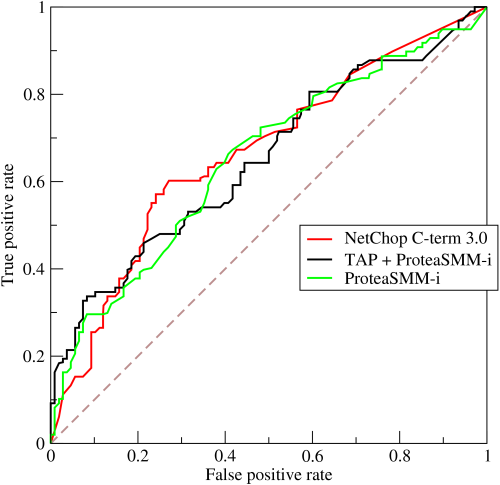
\includegraphics[scale=2]{ROC_Curve.png}
\end{figure}
\\
\noindent
It plots the true positive rate of the classifier against its false positive rate. A single run of the classifier on a set of data would only represent a single point on the plot. However, in practice, we vary the discrimination threshold of the classifier, e.g. the predicted probability for which it predicts a "positive" label, from 1 to 0. For a given classifier this then produces a series of points on the plot, which we connect to form the ROC \textit{curve}. If the threshold probability is 1, all examples are classified as negative and hence both the true and false positive rates are 0. Reducing the threshold probability means more of the true positive labels are correctly predicted as positive - increasing the true positive rate. But this can introduce a higher false positive rate, since more of the true negative labels are predicted as positive. When the threshold reaches 0, all examples are classified as positive, so the true positive rate is 1, but the false positive rate is also 1 since all true negatives are predicted as positive. 
\\
\\
\noindent
However, intermediate points on the ROC curve will indicate the extent to which the classifier can correctly classify positive examples (high true positive rate), while avoiding misclassifying negative examples (low false positive rate). Clearly, a classifier that is better at doing this is preferred, so we prefer those with ROC curves towards the top-left corner of the plot. And a classifier whose ROC curve is strictly above another's in the plot is a strictly better classifier (at least on the given data set).
\\
\\
\noindent
We can summarise this over a whole set of threshold probabilities by calculating the area under the ROC curve, called the \textit{AUC}. A classifier whose ROC curve is strictly above another's will have a larger AUC - so a larger AUC represents a better classifier.

\newpage
\subsection{Model Ensembles}
Look into ensembles of CNN's; move this section above performance measures later.

\newpage
\subsection{State-of-the-Art}
ILSVRC 2017 image classification winner: Squeeze-and-excitation networks https://arxiv.org/abs/1709.01507
Squeeze: global-average pooling over the full height-and-width for each channel of a representation. Results is therefore a scalar for each channel. Seen as capturing the global information about the image carried in each channel ("global information embedding").
Excitation: captures channel-wise dependencies; mutliplies the result of the squeeze op by some new weight matrix W1 (and takes a ReLU). Then dampens this signal by mutliplying the result of that operation by another weight matrix W2 and taking the sigmoid. Size of the weight matrices dictated by number of channels, and some dimension-reduction hyperparameter r. This is again done channel-wise. The result of the sigmoid, s, is then multiplied with the corresponding channel of the original representation, essentially rescaling the original representation. Note s is simply a scalar for each channel.

VGG
Inception
ResNets
MobileNet
ShuffleNet
Attention/Gating


\newpage
\subsection{Pretrained Models}
Discuss the use of pre-trained models - can keep weights the same, replact the head.
Describe the structure of the pre-trained models we'll use for comparison:
[MAYBE PUT INTO APPENDIX?] 
\subsubsection{VGG16}
Describe VGG16 \\

% END BACKGROUND


% BEGIN DATA
\newpage
\section{Data}
Write about the MURA data, show some exmaple images (normal \& abnormal), give data breakdowns 

\subsection{MURA}
Discuss MURA - what it is, how it was produced

\subsection{Image Examples}
As can be seen in \textbf{Figure \ref{fig:xray1}} below, the x-ray is of a hand. A side-profile of the hand from the same study can be seen in \textbf{Figure \ref{fig:xray2}}. \textbf{Figure \ref{fig:xray2_copy}} is a copy of \textbf{Figure \ref{fig:xray2}}.

\begin{figure}
  \centering    
  \caption{Example X-Ray Image}
  \label{fig:xray1}
  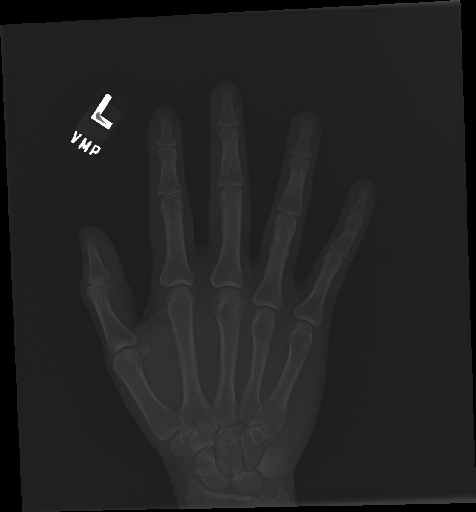
\includegraphics[scale=0.5]{image1.png}
  \caption{Another example X-Ray Image}
  \label{fig:xray2}
  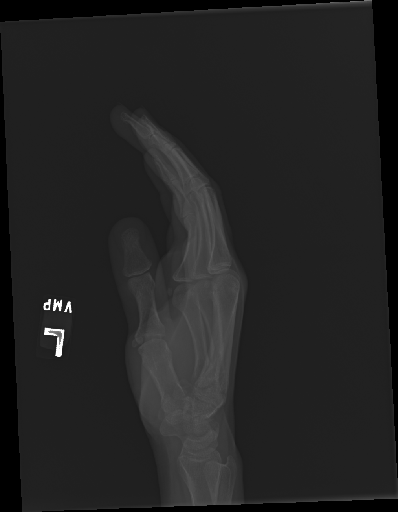
\includegraphics[scale=0.5]{image2.png}
  \caption{A copy of figure 2}
  \label{fig:xray2_copy}
  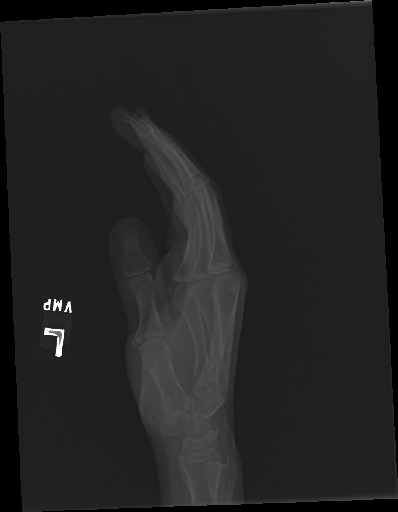
\includegraphics[scale=0.5]{image2_copy.png}
\end{figure}
\clearpage
\noindent

\subsection{Data Breakdowns}
Data breakdowns

% END DATA


% BEGIN MODEL DEVELOPMENT
\newpage
\section{Model Development}

\subsection{Working Environment}
Describe google cloud set-up, GPU, python packages used etc

\subsection{Data Preprocessing}
Describe the preprocessing work done on the data - resize images, normalise values, data augmentation etc 
Random-size cropping?

\subsection{Model}
Describe the final ab-initio model I end up with - structure, loss function, training params/hyperparams etc

\subsection{Predictions}
Discuss getting predictions and aggregating down to study-level predctions

% END MODEL DEVELOPMENT


% BEGIN RESULTS
\newpage
\section{Results}

\subsection{Baseline Performance}
Give the performance of my chosen ab-initio model

\subsection{Image Size}
How do my results vary with size of image? Does increasing image size increase scope for

\subsection{Regularisation}
Perform some regularisation experiments, show results

\subsection{Pre-Trained Models}
How does my model compare vs a selection of pretrained models

% END RESULTS


% BEGIN CONCLUSIONS
\newpage
\section{Conclusions}
Include introspective chapter
Work here not comparable to clinical setting, e.g. smaller, lower resoution images; radiologist may have a relationship with patient - know medical history, other symptoms etc
What is "abnormal"? - type \& severity of abnormality not known, MURA paper not clear.

% END CONCLUSIONS


% BEGIN ETHICAL
\newpage
\section{Professional and Ethical Issues}
Potential Impact on Radiology - Deep Learning tools used to help triage/prioritise radiologists' work, not replace them; 
Can we trust diagnosis to a computer program? Would you be happy to do so? 
Conversely - medical errors happen a lot (est. cost \$X p.a.; any specifics for radiology?) but DL tools may at least help cut that down.

% END ETHICAL


% BEGIN EXTENSIONS
\newpage
\section{Extensions}
Enquire further about what "abnormal" means
Alternative data e.g. CheXNet, others(?)
Alter NN to accept multiple images simultaneously and so predict based on several views at once (e.g. by weight-sharing, or appening all study images into a single 3D tensor)

% END EXTENSIONS



\clearpage
\bibliographystyle{ieeetr}
\bibliography{bibliography}

\clearpage
\appendix
\section{Pretrained Model Architechtures}
Below we describe the architechtures of the various pre-trained neural network models mentioned in the text.
\subsection{VGG16}
This is the VGG16 model.


\end{document}
